\chapter{Results}
In this chapter we examine the rendered output results of our implementation of our BRDF models applied to different input patches such as Blaze grating or Elaphe $\ref{fig:elpahespecies}$ and Xenopeltis $\ref{fig:xenospeicies}$ snake nano-scaled surface sheds. We are discussing and comparing both, their BRDF maps $\ref{fig:brdfmapexplanation}$ and the corresponding renderings on a snake geometry like shown in section $\ref{sec:snakegeomrenderings}$ for various input parameters. Last we also show a real experimental image showing the effect of diffraction for similar parameters like we have.

\section{BRDF maps}
A BRDF map shows a shader's output for all possible viewing directions for a given, fixed, incident light direction. We assume that each viewing direction is expressed in spherical coordinates (See appendix $\ref{sec:sphericalcoordinates}$) $(\theta_v, \phi_v)$ and is represented in the map at point 

\begin{align}
(x,y) = (sin(\theta_v)cos(\phi_v), sin(\theta_v)sin(\phi_v))
\end{align}

with its origin at the map-center. The light direction for normal incidence $(\theta_i, \phi_i)$ has been fixed to $(0,0)$ for our rendered results.

%%TODO replace this graphics by (latest state of paper)
%%TODO add sources!!!!!!!!!!!!!
\begin{figure}[H]
  \centering
  \subfigure[BRDF map schema]{
    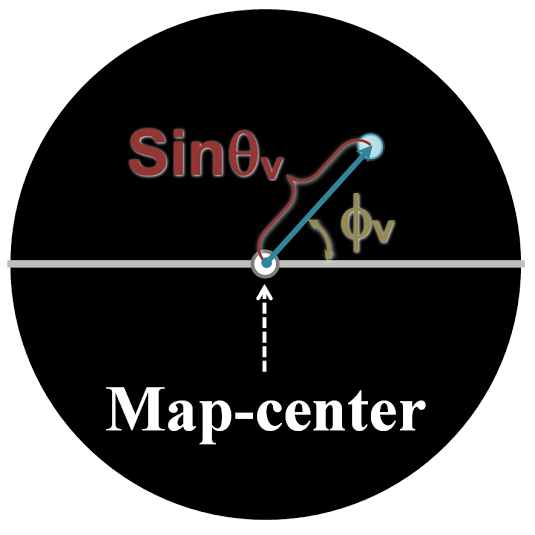
\includegraphics[scale=0.3]{resultsnew/brdfmapschema.png}
    \label{fig:brdfmapschema}
  }
~
  \subfigure[Light reflection geometrical setting]{
    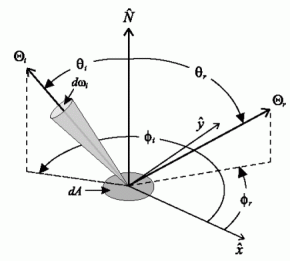
\includegraphics[scale=0.7]{results/Lightreflectiongeometry.png}
    \label{fig:lightreflectiongeometry}
  }
~

\caption[BRDF Map]{BRDF maps$\footnotemark$ for different patches: $\Theta=(\theta_i,\phi_i)$ is the direction of light propagation}
\label{fig:brdfmapexplanation}
\end{figure}
\footnotetext{image source of figure:
\begin{itemize}
  \item \ref{fig:brdfmapschema}: Taken from D.S.Dhillon's Paper $\cite{daljitpaper}$
  \item \ref{fig:lightreflectiongeometry}: Taken from \texttt{http://math.nist.gov/\textasciitilde FHunt/appearance/brdf.html}
  \end{itemize}
}

%%TODO maybe add glue fun - refere to schematics.
%%TODO say something about used gratings.

\begin{figure}[H]
  \centering
  \subfigure[Blaze grating with scale of 2.500 $\mu m$]{
    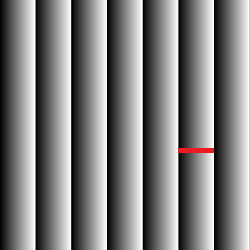
\includegraphics[scale=0.5]{evaluation/blaze_res.png}
    \label{fig:blazegratingpatch}
  }
~
  \subfigure[Elaphe patch with scale of 3.270 $\mu m$]{
    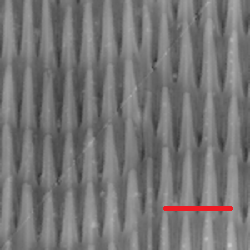
\includegraphics[scale=0.5]{evaluation/elaphe_res.png}
    \label{fig:elpahegratingpatch}
  }
~
  \subfigure[Xenopeltis patch with scale of 3.210 $\mu m$]{
    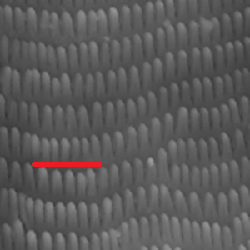
\includegraphics[scale=0.5]{evaluation/xeno_res.png}
    \label{fig:xenogratingpatch}
  }

\caption[Our Gratings]{Cutouts of our nano-scaled surface gratings used for rendering within our shader with a scale indicator (red line) for each patch. Note that for rendering, we use larger patches.}
\label{fig:gratingpatches}
\end{figure}

Figure $\ref{fig:brdfmapsdiffpatches}$ shows the BRDF maps of the full lambda space sampling approach (\textbf{FLSS}) as described in section $\ref{sec:fragmentshader}$ applied on different nanoscale surface gratings as shown in figure $\ref{fig:gratingpatches}$. In Subfigure $\ref{fig:brdfmapBlaze}$ we see the BRDF map for the Blazed grating, showing high relative brightness for its first order diffraction, i.e. for the Blazed gratings most of the diffracted spectral energy lies in its first order. Note that for Blazed grating their first-order diffracted light returns along the same path as the incident light. Higher diffraction modes are still perceivable (second and higher diffraction orders) but with a much lower relative brightness. The asymmetry of the pattern is due to the asymmetric geometry of the grating $\ref{fig:blazegratingpatch}$. \\

The finger-like structures contained in the Elaphe surface grating $\ref{fig:elpahegratingpatch}$ are quite regularly aligned and hence diffraction occurs along the horizontal axis for the BRDF map as shown in figure $\ref{fig:brdfmapElaphe}$. The reason for not seeing any strong diffraction color contribution along other directions in the BRDF map is due to the fact that these ‘nano-fingers’ overlap across layers and thus do not exhibit any well-formed periodicity along finger direction. \\

For Xenopeltis surface grating $\ref{fig:xenogratingpatch}$, we observe diffraction along many different, almost vertical directions in the BRDF map $\ref{fig:brdfmapXeno}$ since the layers of the finger-like structures do not overlap and are shifted significantly along their length but still exhibit some local consistency. A similar argument holds true for diffraction across locally periodic finger patches with slightly different orientations. 

\begin{figure}[H]
  \centering
  \subfigure[Blazed grating]{
    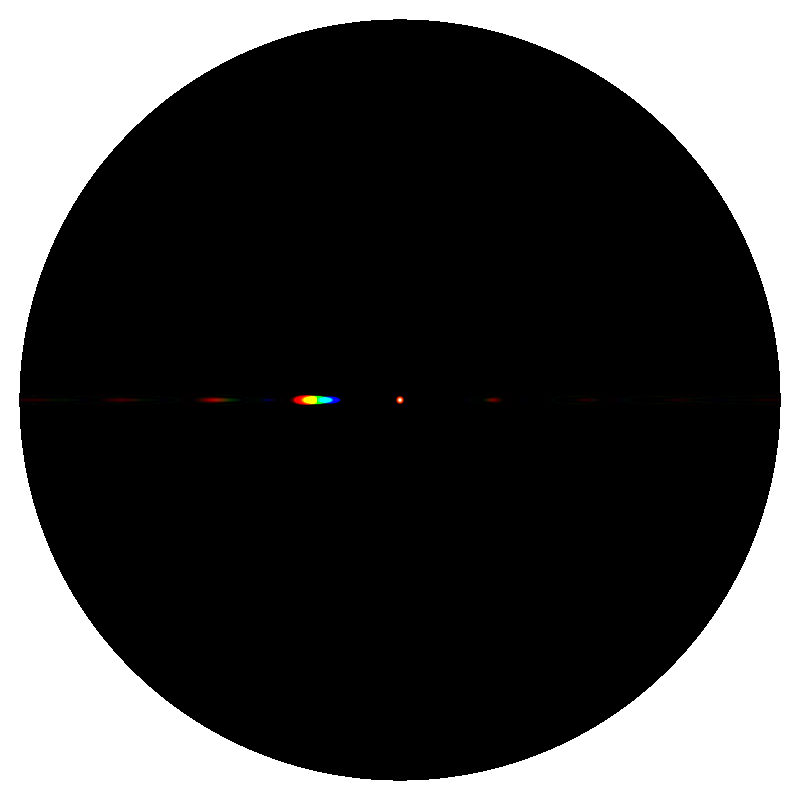
\includegraphics[scale=0.12]{results/diffPatches/fftBlazeHeight_0.25Microns_allL_weak_scale.png}
    \label{fig:brdfmapBlaze}
  }
~
  \subfigure[Elaphe grating]{
    \includegraphics[scale=0.12]{results/diffPatches/elaph65.png}
    \label{fig:brdfmapElaphe}
  }
~
  \subfigure[Xenopeltis grating]{
    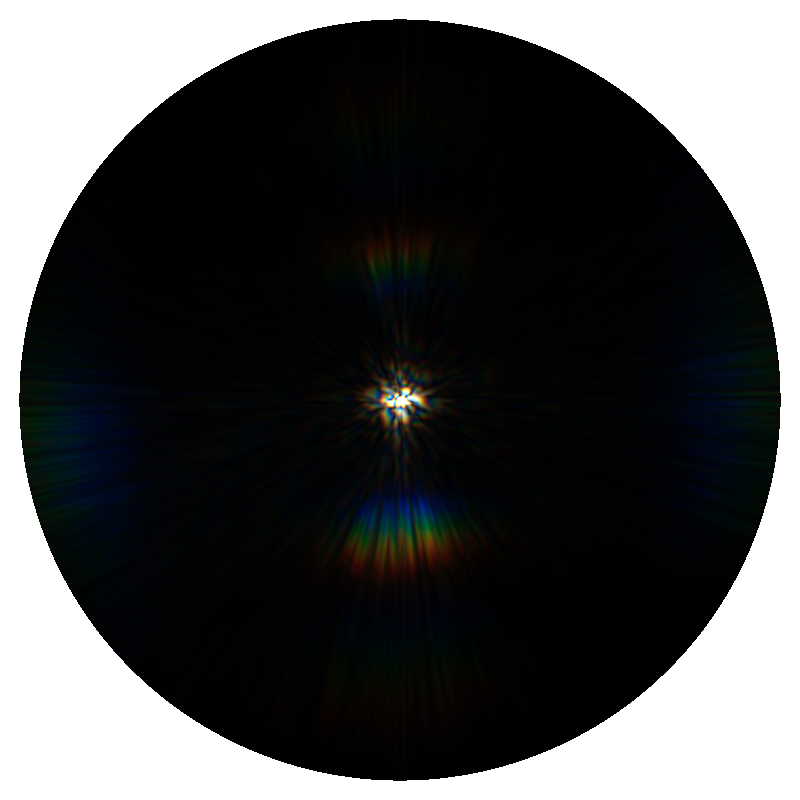
\includegraphics[scale=0.12]{results/diffPatches/xeno65.png}
    \label{fig:brdfmapXeno}
  }

\caption[BRDF Map FLSS of our Gratings]{BRDF maps for different patches}
\label{fig:brdfmapsdiffpatches}
\end{figure}

%%TODO eplain what gound truth is refering to, what it is supposed to denote.

Figure $\ref{fig:brdfmapsdiffrenderingapproaches}$ shows BRDF maps of all our BRDF models applied on the Blaze grating. Figure $\ref{fig:brdfmapblazeallLambda}$ shows the FLSS shading approach result for our blazed grating and it is used in order to compare with our other rendering approaches. \\

%%TODO intruduce somehere NMM approach $N_{min}, N_{max}$
Figure $\ref{fig:brdfmapblazeonlyreq}$ shows the BRDF map for the NMM approach which is close to the FLSS approach, verified in section $\ref{sec:approachesverifications}$, just like in the case of corresponding evaluation plots $\ref{fig:blazneval}$ already were closely matching. Nevertheless there is a small, noticable difference: 

%TODO: rework this: first explain differences and them apply the reasoning.
since in the actual technical implementation of the NMM shading approach treats the center of the BRDF map as a separate case, i.e. everything around a small $\epsilon$-circumference has white color assigned we note a white circular spot around the map center. Except this fact, the BRDF map resembles the FLSS results. \\
%% end unsafe

Figure $\ref{fig:brdfmapblazepq}$ shows the BRDF map for the PQ approach which relies on sinc-interpolation. The PQ BRDF map and the FLSS results are visual alike. Compared to the evaluation plots, the PQ BRDF maps even persuade more. One difference we notice is that the first order is a little spread. This effect is would be strengthened when using linear interpolation instead of sinc-interpolation. \\

Last, let us consider figure $\ref{fig:brdfmapblazegem}$ which shows the BRDF map produced by using the implementation of Nvidia Gem's implementation (ADD REFERENCE) of Stam's BRDF model, when constrainting the y-axisis of the BRDF map. This model does not consider much more than the spacing $d$ of a given grating. It also always produces highly symmetric results. It also does not render different orders of diffraction rather than the zero and first order.   

% brdf maps patches
\begin{figure}[H]
  \centering
  \subfigure[FLSS]{
    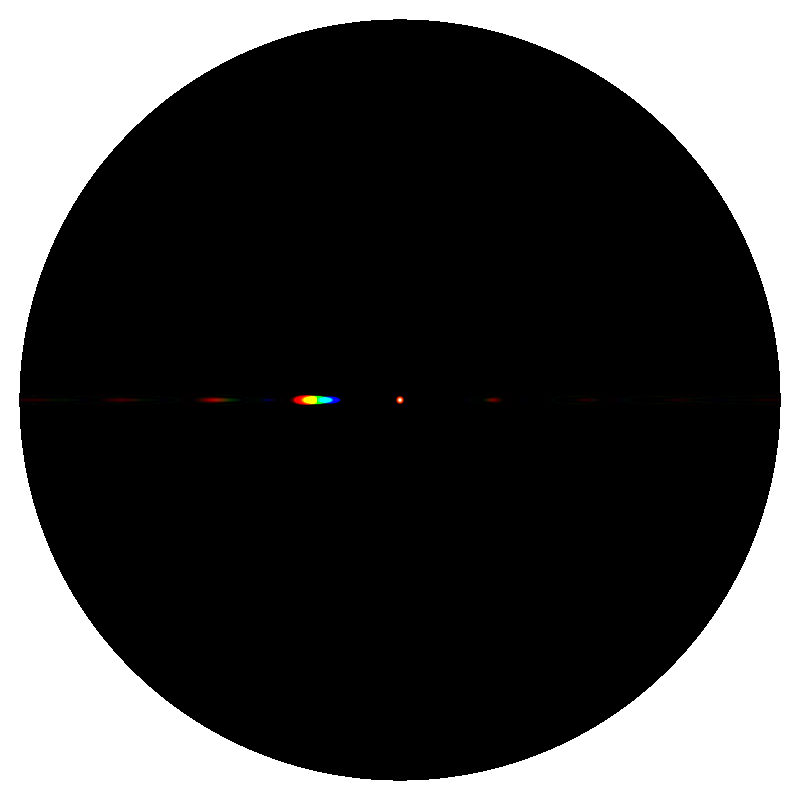
\includegraphics[scale=0.09]{results/diffPatches/fftBlazeHeight_0.25Microns_allL_weak_scale.png}
    \label{fig:brdfmapblazeallLambda}
  }
~
  \subfigure[NMMS]{
    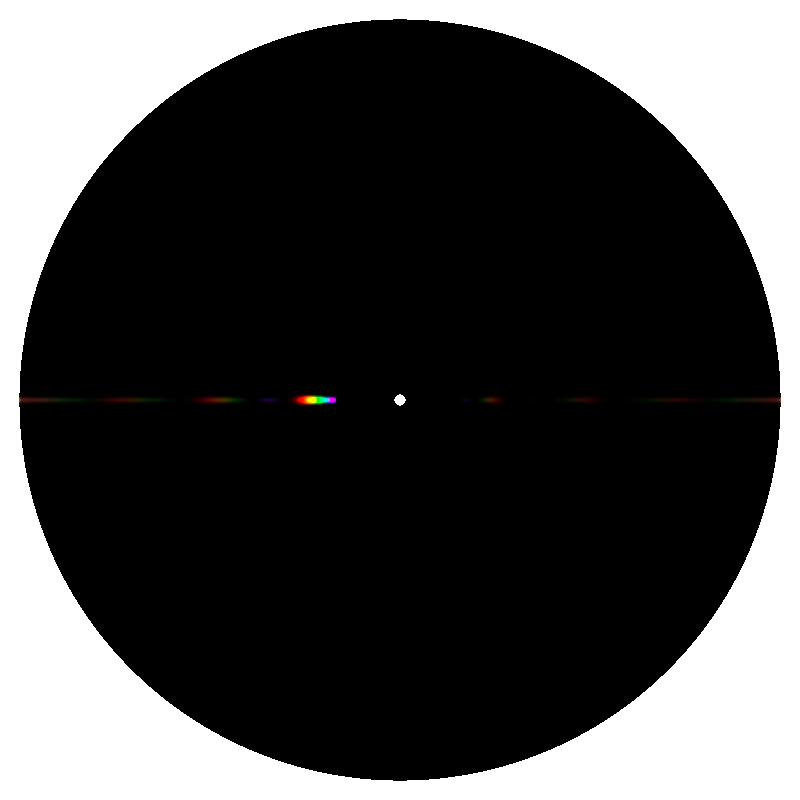
\includegraphics[scale=0.09]{results/methodComp/blazedNMMS.png}
    \label{fig:brdfmapblazeonlyreq}
  }
~
  \subfigure[PQ with Sinc-Interpolation]{
    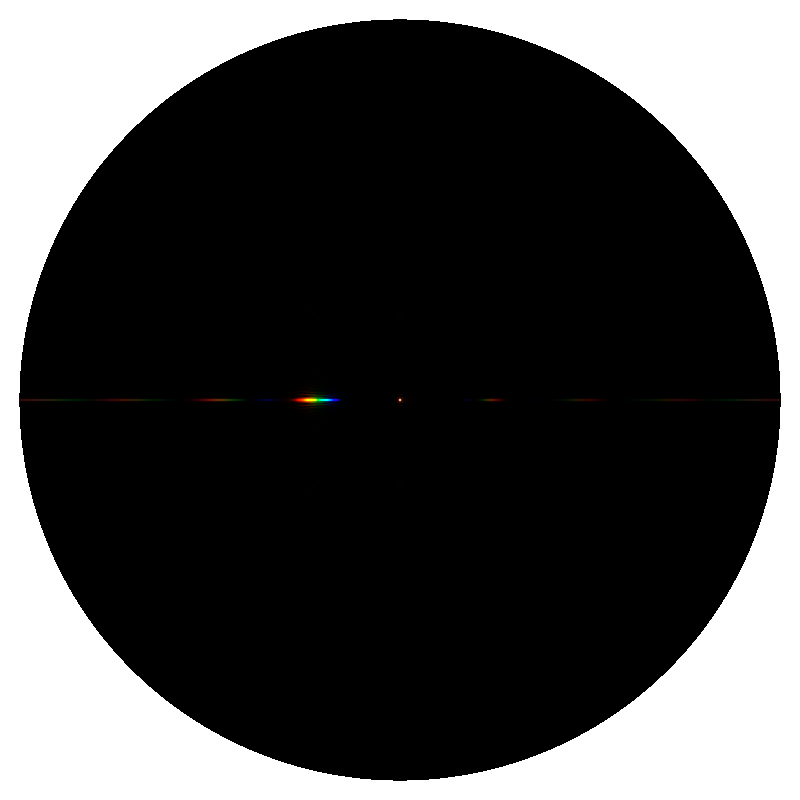
\includegraphics[scale=0.09]{results/methodComp/pqsincinterpol}
    \label{fig:brdfmapblazepq}
  }
~
  \subfigure[Nvidia Gem's Approach]{
    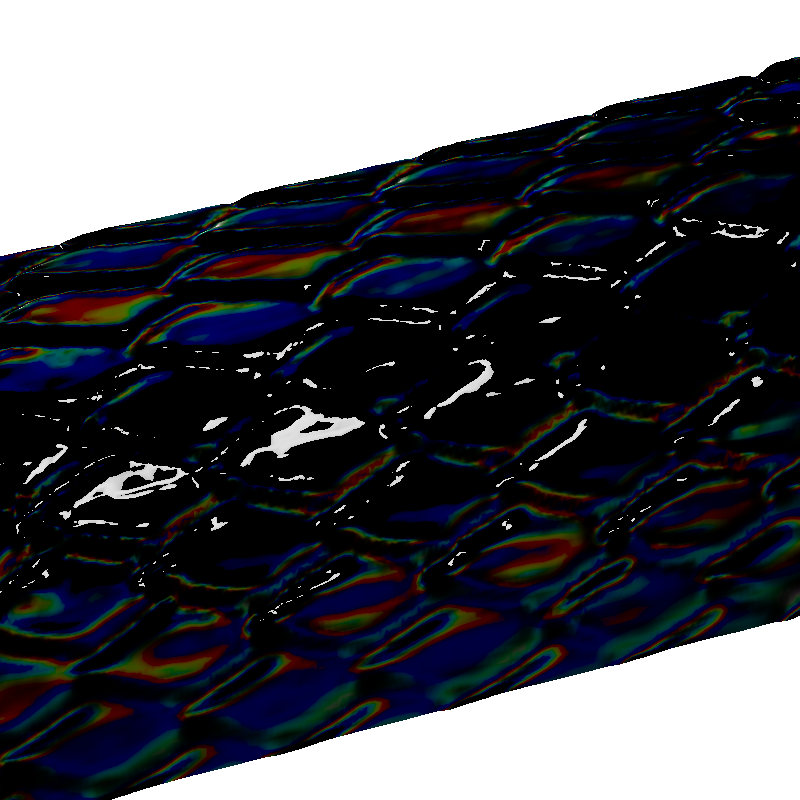
\includegraphics[scale=0.09]{results/methodComp/gem.png}
    \label{fig:brdfmapblazegem}
  }
    
\caption[BRDF Map using our Approaches for Blazed Grating]{BRDF maps for Blazed grating comparing our different rendering approaches}
\label{fig:brdfmapsdiffrenderingapproaches}
\end{figure}

Figure $\ref{fig:brdfmapsdifflambdastepsblaze}$ and figure $\ref{fig:brdfmapsdifflambdastepselaphe65}$ show the BRDF maps for different wavelength step sizes used in the fragment shader for the full lambda space sampling approach applied on the Blaze grating and the Elpahe snake shed, respectively. Within our fragment shaders the most outer loop iterate over the range $[380nm, 780nm]$ for fixed step sizes $\lambda_{step}$ which basically constitutes the integration over the wavelength spectrum. Therefore, having bigger step sizes implies having fewer step sizes which will fasten up the overall runtime of a shader but will also introduce artifacts and therefore lower the overall shading qualtity. For Elaphe surface grating, artifacts are perceptional arising when $\lambda_{step} \leq 10nm$. Results produced by using $5nm$ step sizes do not differ from those produced by using $\lambda_{step}= 1nm$ which allows us to set $\lambda_{step}$ equal 5nm. For a Blazed grating we may chose even bigger step sized without losing any rendering quality.   

% blaze steps
\begin{figure}[H]
  \centering
  \subfigure[$\lambda_{step=1 nm}$]{
    \includegraphics[scale=0.12]{results/different_lambda_steps/blaze/dl=1.png}
    \label{fig:brdfmapsDiffLambdaStepsL1Blaze}
  }
~
  \subfigure[$\lambda_{step=5 nm}$]{
    \includegraphics[scale=0.12]{results/different_lambda_steps/blaze/dl=5.png}
    \label{fig:brdfmapsDiffLambdaStepsL5Blaze}
  }
~
  \subfigure[$\lambda_{step=10 nm}$]{
    \includegraphics[scale=0.12]{results/different_lambda_steps/blaze/dl=10.png}
    \label{fig:brdfmapsDiffLambdaStepsL10Blaze}
  }
  
  \subfigure[$\lambda_{step=25 nm}$]{
    \includegraphics[scale=0.12]{results/different_lambda_steps/blaze/dl=25.png}
    \label{fig:brdfmapsDiffLambdaStepsL25Blaze}
  }
~
  \subfigure[$\lambda_{step=50 nm}$]{
    \includegraphics[scale=0.12]{results/different_lambda_steps/blaze/dl=50.png}
    \label{fig:brdfmapsDiffLambdaStepsL50Blaze}
  }
~ 
  \subfigure[$\lambda_{step=100 nm}$]{
    \includegraphics[scale=0.12]{results/different_lambda_steps/blaze/dl=100.png}
    \label{fig:brdfmapsDiffLambdaStepsL100Blaze}
  }
  
\caption[BRDF Map varying step sizes FLSS Blazed Grating]{Blazed grating at $2.5 \mu m$: Different $\lambda$ step sizes}
\label{fig:brdfmapsdifflambdastepsblaze}
\end{figure}

% elpahe steps
\begin{figure}[H]
  \centering
  \subfigure[$\lambda_{step=1 nm}$]{
    \includegraphics[scale=0.12]{results/different_lambda_steps/elaphe65/dl=1.png}
    \label{fig:brdfmapsDiffLambdaStepsL1Elaphe65}
  }
~
  \subfigure[$\lambda_{step=5 nm}$]{
    \includegraphics[scale=0.12]{results/different_lambda_steps/elaphe65/dl=5.png}
    \label{fig:brdfmapsDiffLambdaStepsL5Elaphe65}
  }
~
  \subfigure[$\lambda_{step=10 nm}$]{
    \includegraphics[scale=0.12]{results/different_lambda_steps/elaphe65/dl=10.png}
    \label{fig:brdfmapsDiffLambdaStepsL10Elaphe65}
  }
  
  \subfigure[$\lambda_{step=25 nm}$]{
    \includegraphics[scale=0.12]{results/different_lambda_steps/elaphe65/dl=25.png}
    \label{fig:brdfmapsDiffLambdaStepsL25Elaphe65}
  }
~
  \subfigure[$\lambda_{step=50 nm}$]{
    \includegraphics[scale=0.12]{results/different_lambda_steps/elaphe65/dl=50.png}
    \label{fig:brdfmapsDiffLambdaStepsL50Elaphe65}
  }
~ 
  \subfigure[$\lambda_{step=100 nm}$]{
    \includegraphics[scale=0.12]{results/different_lambda_steps/elaphe65/dl=100.png}
    \label{fig:brdfmapsDiffLambdaStepsL100Elaphe65}
  }
  
\caption[BRDF Map varying step sizes FLSS Elaphe Grating]{Elaphe grating at $65 \mu m$: Different $\lambda$ step sizes}
\label{fig:brdfmapsdifflambdastepselaphe65}
\end{figure}


The Figures $\ref{fig:pqblaze}$, $\ref{fig:pqxeno}$, $\ref{fig:pqelaphe}$ show a comparison of the BRDF maps produced by full lambda space sampling approach (on the left) and the PQ shading approach (on the right) applied on all our patches. For Blazed grating, as already mentioned, we notice that both approaches resemble each other. We also notice that for PQ map, the first order diffraction color contribution is spread. For Elaphe and Xenopeltis grating we notice similar shaped BRDF patterns, even when the angle of light varies, but nevertheless, they also contain some artifacts. This also holds true when we linearly interpolate instead relying on sinc-interpolation.

%pq blaze
\begin{figure}[H]
  \centering
  \subfigure[Full Lambda Sampling: Blazed grating]{
    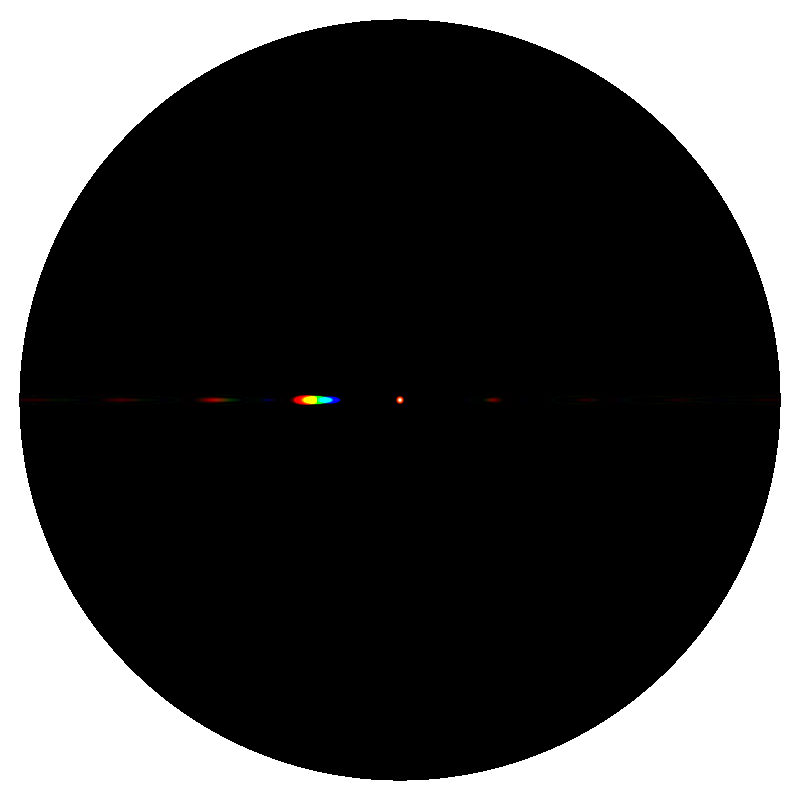
\includegraphics[scale=0.12]{results/PQapproach_vs_sampleAll/blaze/fftBlazeHeight_0.25Microns_allL_weak_scale_g=1.1.png}
    \label{fig:fullLambdaBlaze}
  }
~
  \subfigure[Full Lambda Sampling brightened: Blazed grating]{
            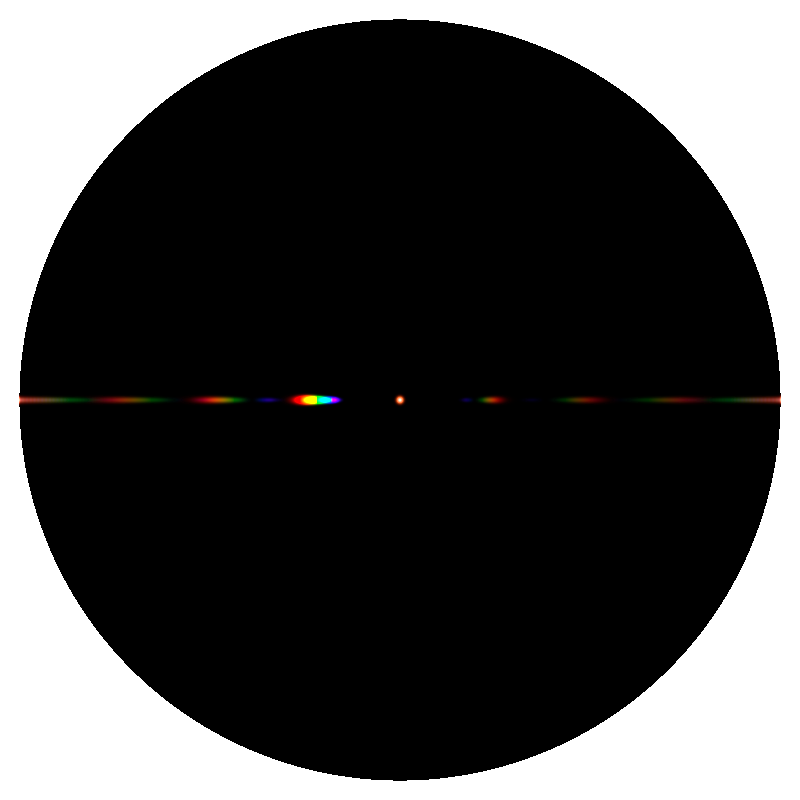
\includegraphics[scale=0.12]{results/PQapproach_vs_sampleAll/blaze/fftBlazeHeight_0.25Microns_allL_weak_scale_g=2.2_scale=100.png}
    \label{fig:fullLambdaBrightenedBlaze}
  }
~
  \subfigure[PQ Approach: Blazed grating]{
    \includegraphics[scale=0.12]{results/PQapproach_vs_sampleAll/blaze/pq.png}
    \label{fig:pqBlaze}
  }
  
\caption{Blazed grating: PQ approach vs full lambda space sampling}
\label{fig:pqblaze}
\end{figure}

%pq elaphe
\begin{figure}[H]
  \centering
  \subfigure[Full Lambda Sampling: Elaphe grating]{
    \includegraphics[scale=0.2]{results/PQapproach_vs_sampleAll/elaphe/elaph65.png}
    \label{fig:fullLambdaElaphe}
  }
~
  \subfigure[PQ Approach: Elaphe grating]{
    \includegraphics[scale=0.2]{results/PQapproach_vs_sampleAll/elaphe/pq.png}
    \label{fig:pqElaphe}
  }

  
\caption{Elaphe grating: PQ approach vs full lambda space sampling}
\label{fig:pqelaphe}
\end{figure}

%pq xeno
\begin{figure}[H]
  \centering
  \subfigure[Full Lambda Sampling: Xeno grating $\theta_i = 0 degree$]{
    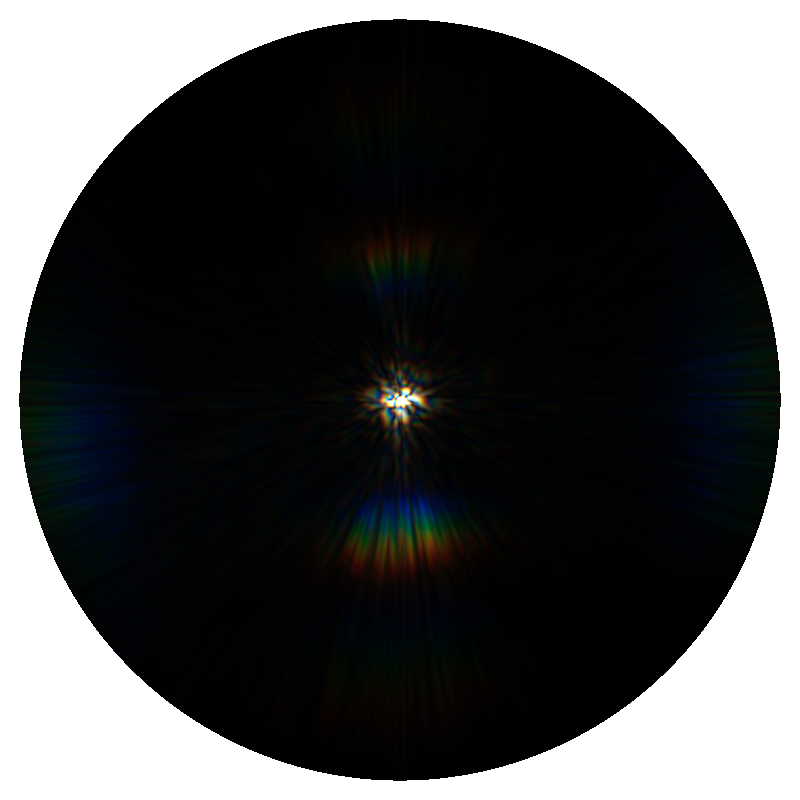
\includegraphics[scale=0.19]{results/PQapproach_vs_sampleAll/xeno/a_xeno_t_i=0.png}
    \label{fig:fullLambdaXenoti0}
  }
~
  \subfigure[PQ Approach: Xeno grating $\theta_i = 0 degree$]{
    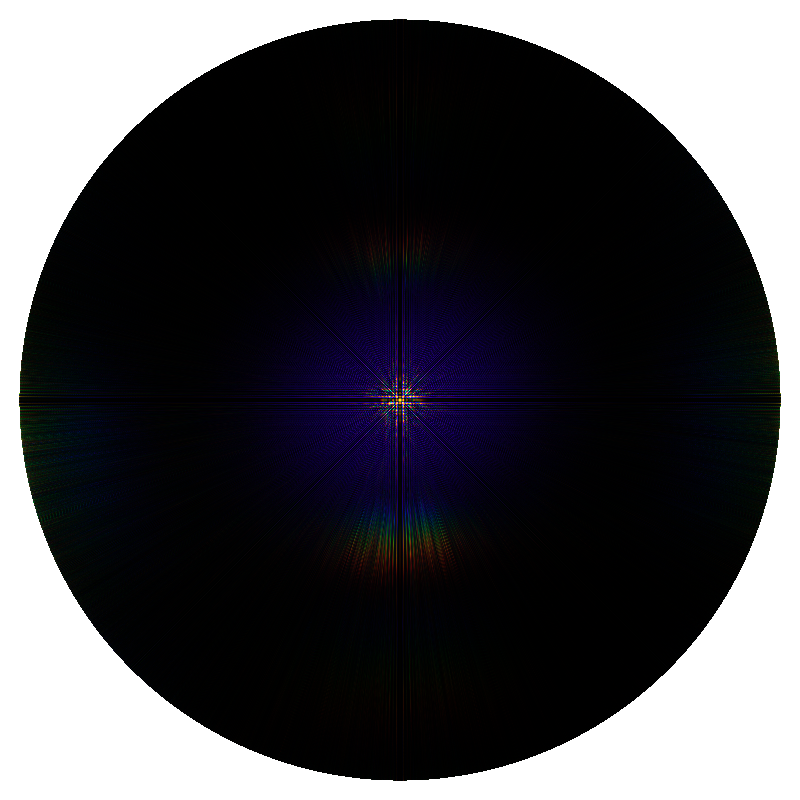
\includegraphics[scale=0.19]{results/PQapproach_vs_sampleAll/xeno/a_pq_t_i=0.png}
    \label{fig:pqXenoti0}
  }

  \subfigure[Full Lambda Sampling: Xeno grating $\theta_i = 10 degree$]{
    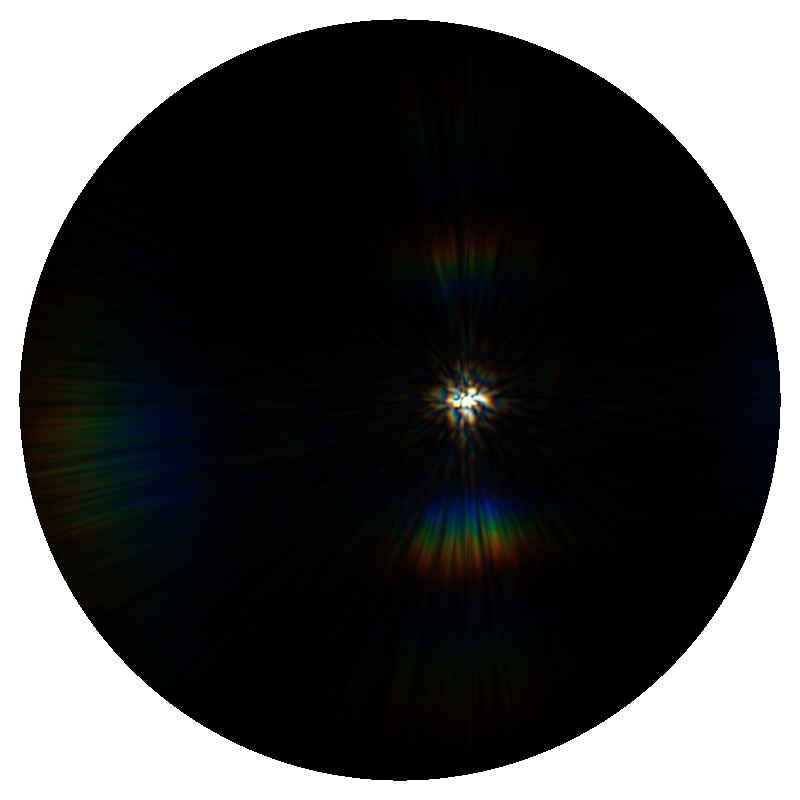
\includegraphics[scale=0.19]{results/PQapproach_vs_sampleAll/xeno/b_xeno_t_i=10.png}
    \label{fig:fullLambdaXenoti10}
  }
~
  \subfigure[PQ Approach: Xeno grating $\theta_i = 10 degree$]{
    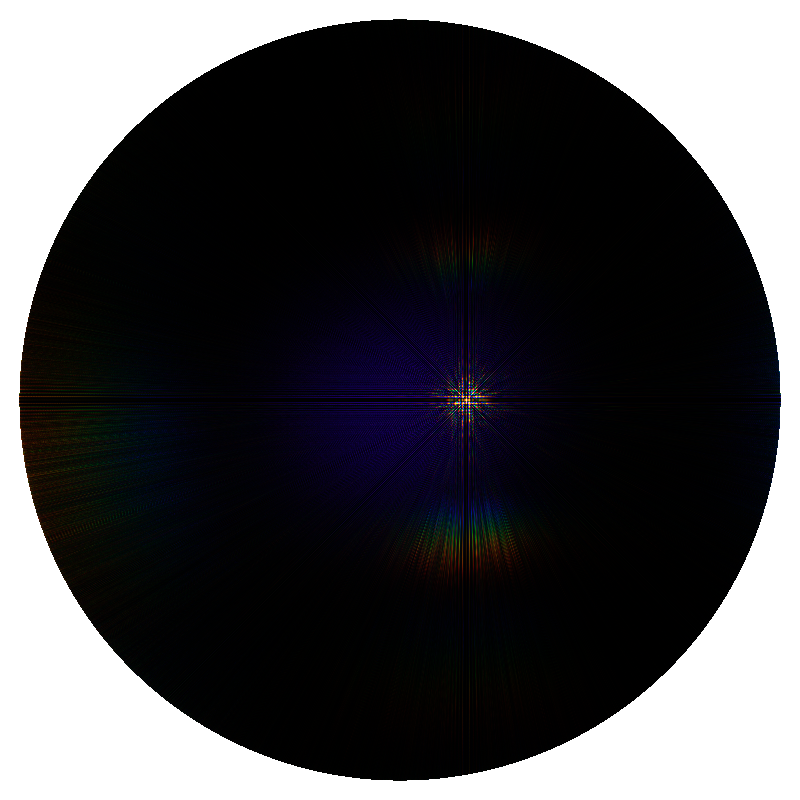
\includegraphics[scale=0.19]{results/PQapproach_vs_sampleAll/xeno/b_pq_t_i=10.png}
    \label{fig:pqXenoti10}
  }
  
  \subfigure[Full Lambda Sampling: Xeno grating $\theta_i = 20 degree$]{
    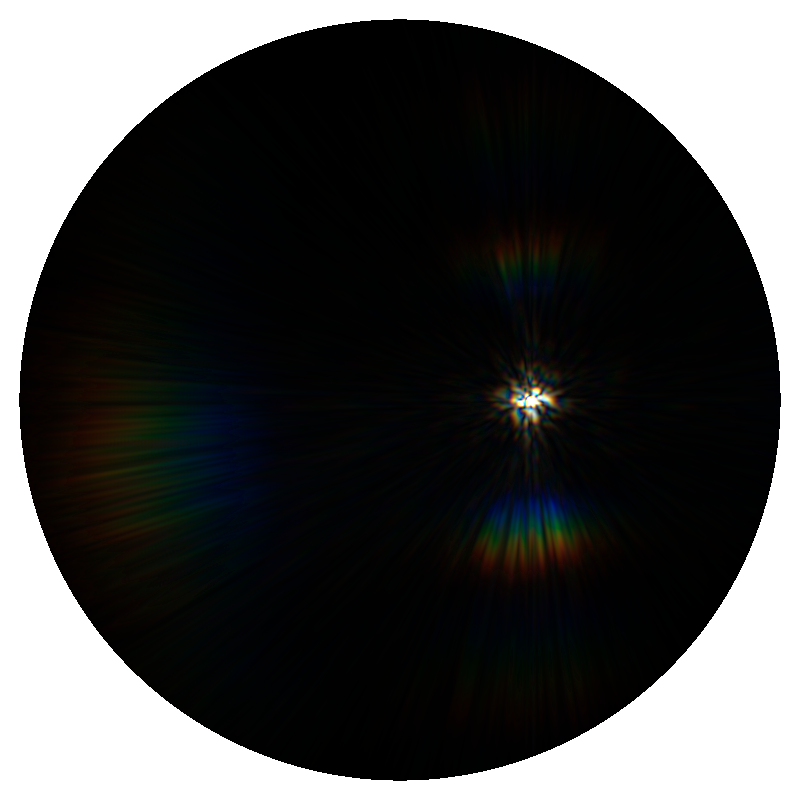
\includegraphics[scale=0.19]{results/PQapproach_vs_sampleAll/xeno/c_xeno_t_i=20.png}
    \label{fig:fullLambdaXenoti20}
  }
~
  \subfigure[PQ Approach: Xeno grating $\theta_i = 20 degree$]{
    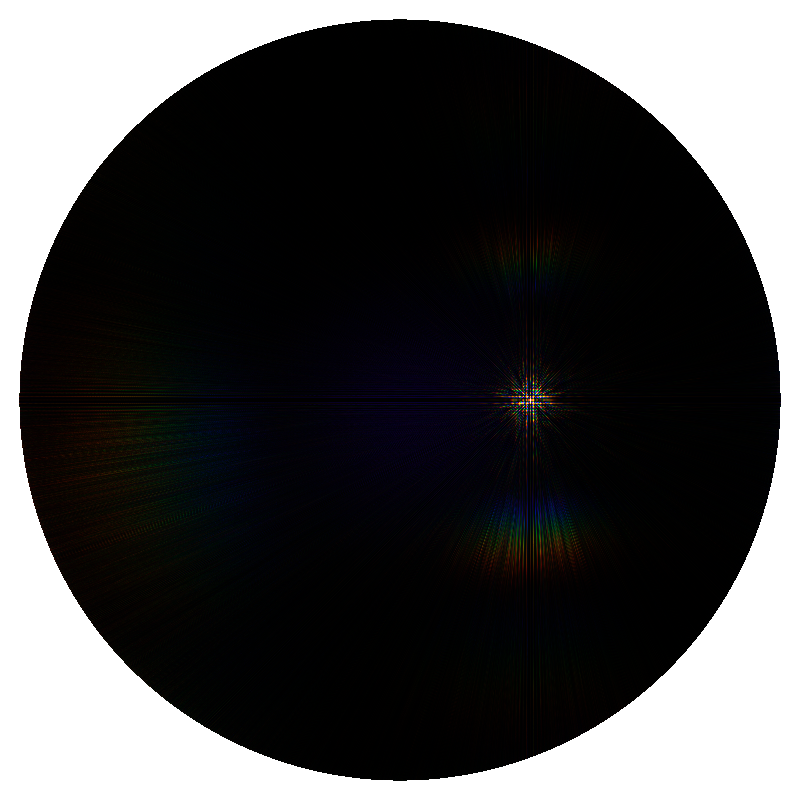
\includegraphics[scale=0.19]{results/PQapproach_vs_sampleAll/xeno/c_pq_t_i=20.png}
    \label{fig:pqXenoti20}
  }
  
\caption{Xeno grating: PQ approach vs full lambda space sampling}
\label{fig:pqxeno}
\end{figure}

Figure $\ref{fig:brdfmapsdiffsigmasizeblaze}$ shows BRDF map for the full lambda sampling approach applied on the Blazed grating, varying the value for the spacial variance $\sigma_s$. This is similar to consider the output of different coherence lengths for our incident light. The lower the coherence length, the fewer interacting grating periods produce produce blurred diffraction bands for different $\lambda$ which overlap to produce poorly resolved colors.

%sigma var
\begin{figure}[H]
  \centering
  \subfigure[$\sigma_{s=3.25 \mu m}$]{
    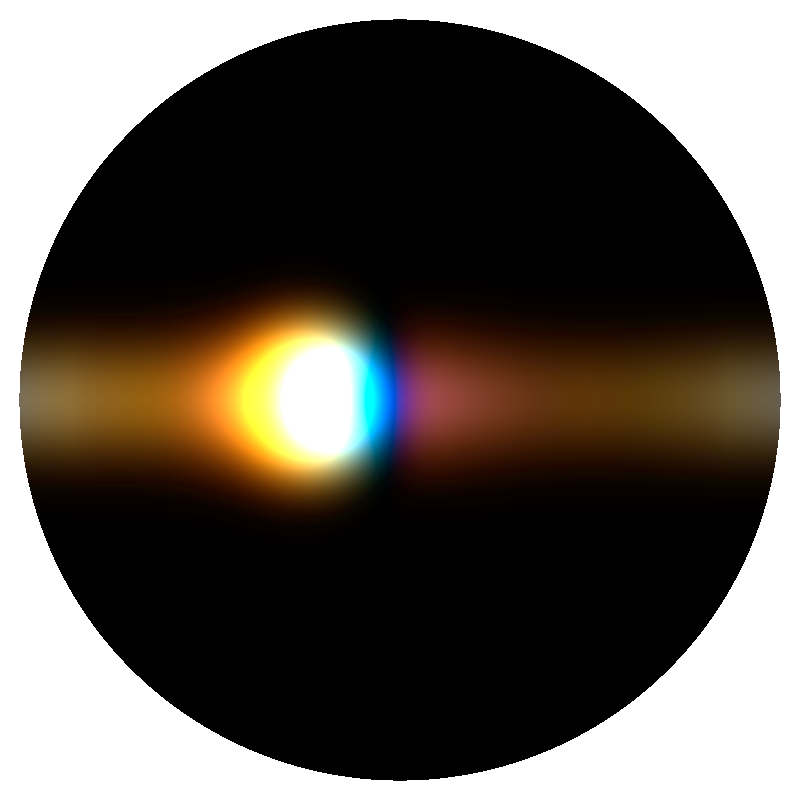
\includegraphics[scale=0.12]{results/sigma_sVariation/blaze/sigma_s=3.25.png}
    \label{fig:brdfmapsDiffSigmaStepsL1Blaze}
  }
~
  \subfigure[$\sigma_{s=6.5 \mu m}$]{
    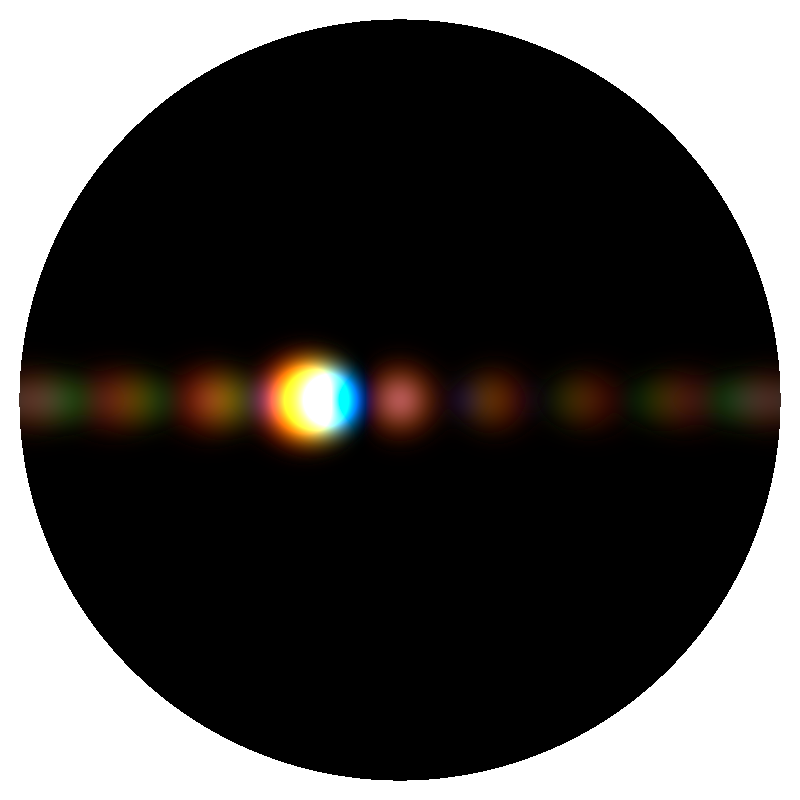
\includegraphics[scale=0.12]{results/sigma_sVariation/blaze/sigma_s=6.5.png}
    \label{fig:brdfmapsDiffSigmaStepsL5Blaze}
  }
~
  \subfigure[$\sigma_{s=15 \mu m}$]{
    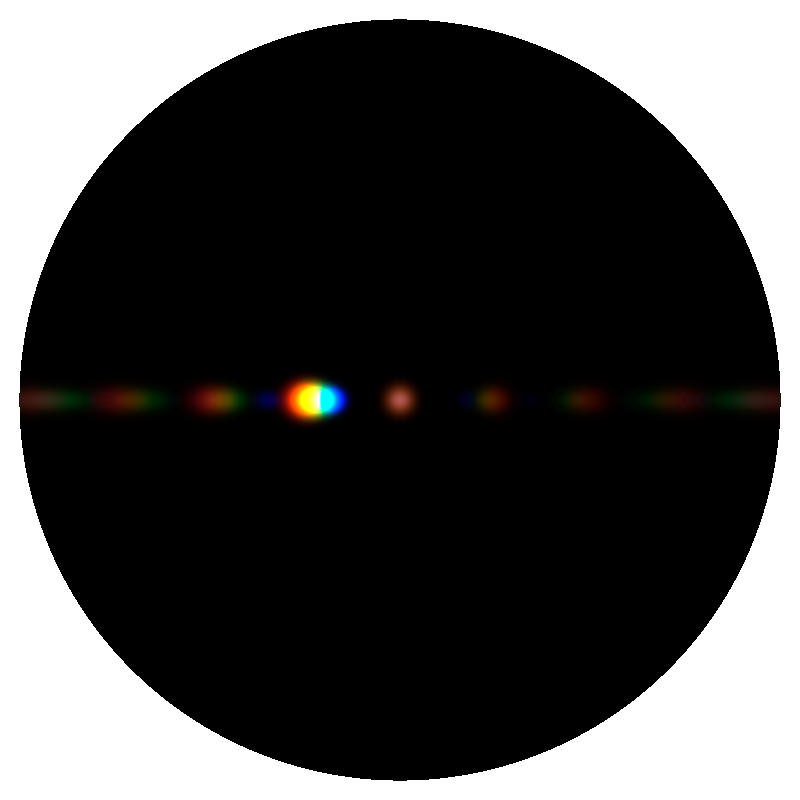
\includegraphics[scale=0.12]{results/sigma_sVariation/blaze/sigma_s=15.png}
    \label{fig:brdfmapsDiffSigmaStepsL10Blaze}
  }
  
  \subfigure[$\sigma_{s=30 \mu m}$]{
    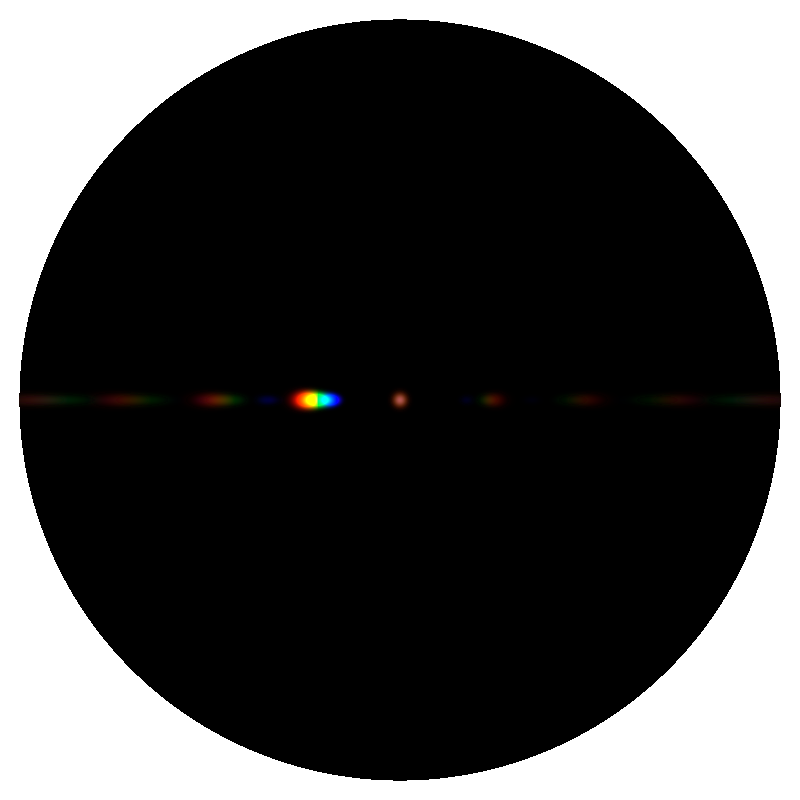
\includegraphics[scale=0.12]{results/sigma_sVariation/blaze/sigma_s=30.png}
    \label{fig:brdfmapsDiffSigmaStepsL25Blaze}
  }
~
  \subfigure[$\sigma_{s=45 \mu m}$]{
    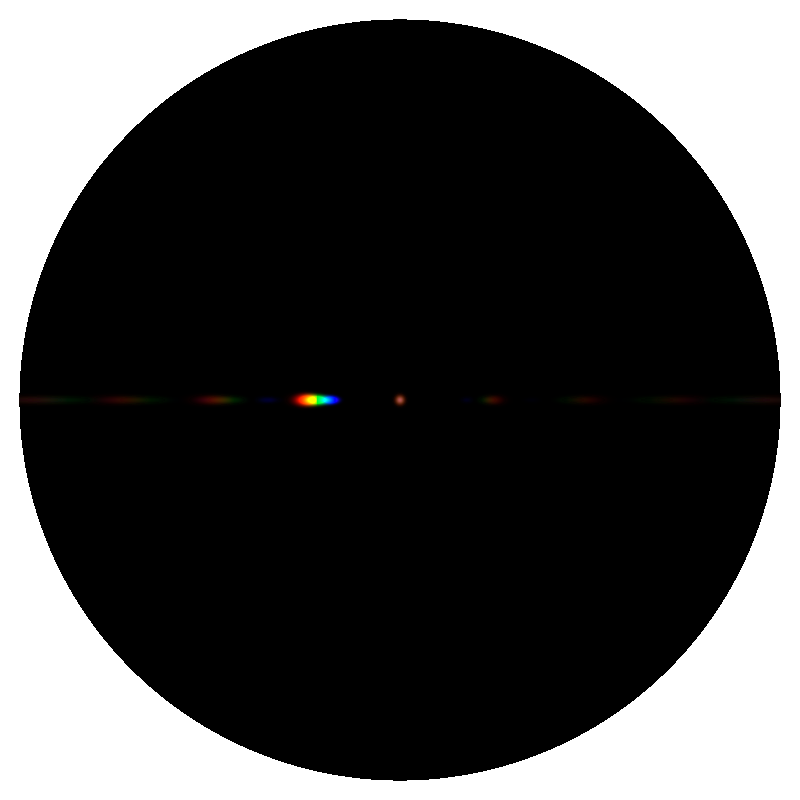
\includegraphics[scale=0.12]{results/sigma_sVariation/blaze/sigma_s=45.png}
    \label{fig:brdfmapsDiffSigmaStepsL50Blaze}
  }
~ 
  \subfigure[$\sigma_{s=65 \mu m}$]{
    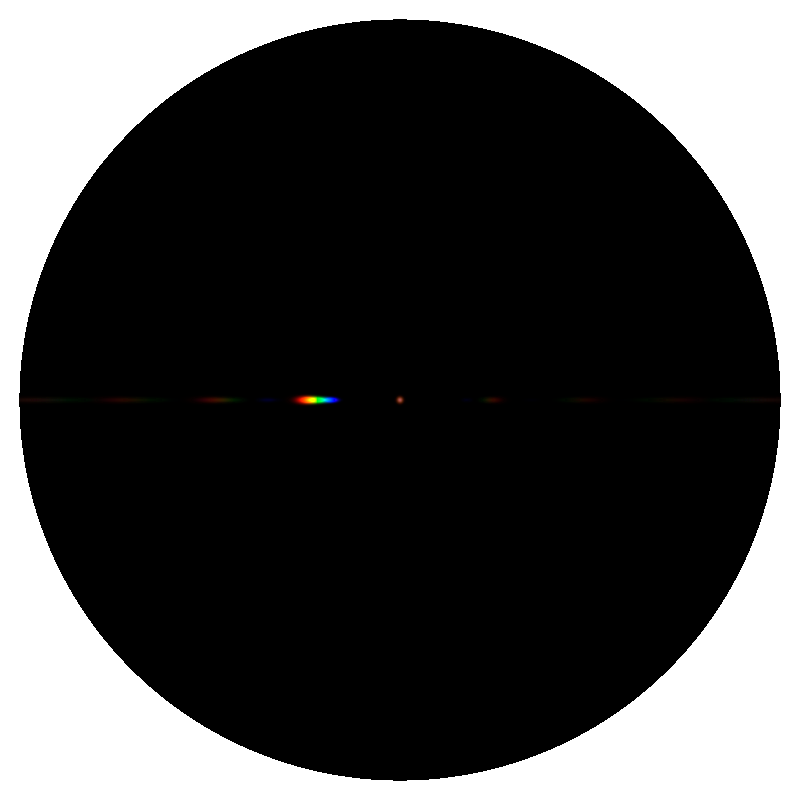
\includegraphics[scale=0.12]{results/sigma_sVariation/blaze/sigma_s=65.png}
    \label{fig:brdfmapsDiffSigmaStepsL100Blaze}
  }
  
  
\caption{Blazed grating at $2.5 \mu m$: Different $\sigma_s$ sizes}
\label{fig:brdfmapsdiffsigmasizeblaze}
\end{figure}

The figures $\ref{fig:brdfmapstayloriterationsblaze}$ and $\ref{fig:brdfmapstayloriterationselaphe65}$ show the BRDF maps of the full lambda space approach using different values for $N$ used for the taylor series approximation used within our fragment shaders. For both input patches we clearly visually observe the convergence of the taylor series for higher values for N.
We visually observe convergence of the Taylor series for all our from a certain value of $N$. In section $\ref{sec:taylorapproximation}$ we already provided a proof for the convergence for a specific geometrical set up which could be applied easily to another setup. The higher the value of $N$ the less the BRDF map changes. For the Blazed grating, we do not see much changing patterns for $N \geq 7$ and for the Elaphe surface grating $N \geq 9$. In general it is rather hard to say for what value of $N$ we have visual convergence since in algorithm $\ref{alg:matlabprecomp}$ we compute the inverse FFT of $power(1j*patchImg, t)$ which is equivalent to $iFFT(patchImg)^n \cdot i^n$. Since we multiply this by $i^n$ there are four possible series where each converges within its own convergence radius.

%taylor var blaze
\begin{figure}[H]
  \centering
  \subfigure[$N=0$]{
    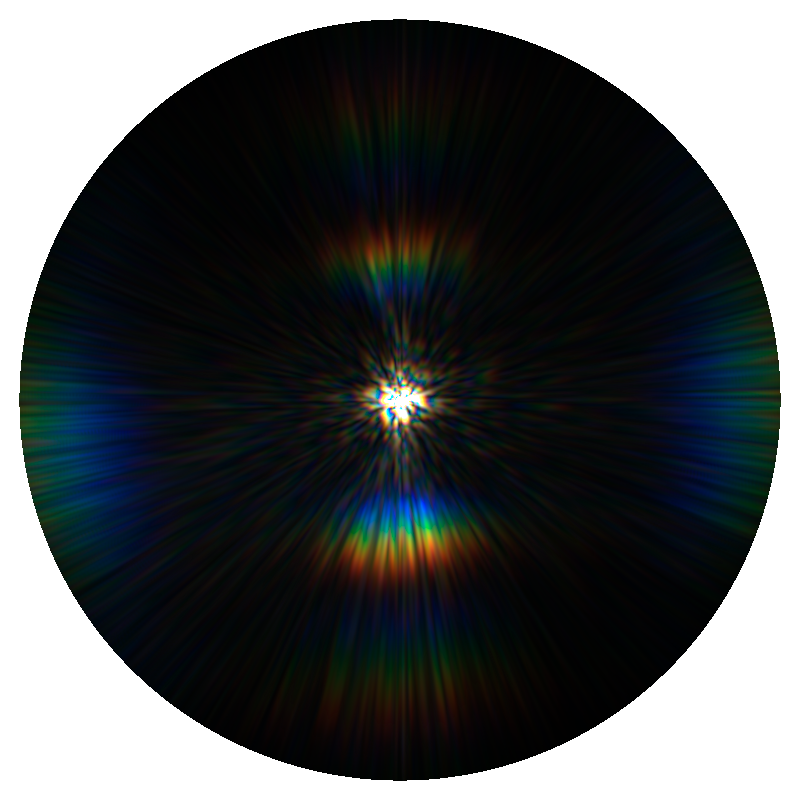
\includegraphics[scale=0.06]{results/taylorStepsVar/blaze/0.png}
    \label{fig:brdfmapsTaylorN0Blaze}
  }
~
  \subfigure[$N=1$]{
    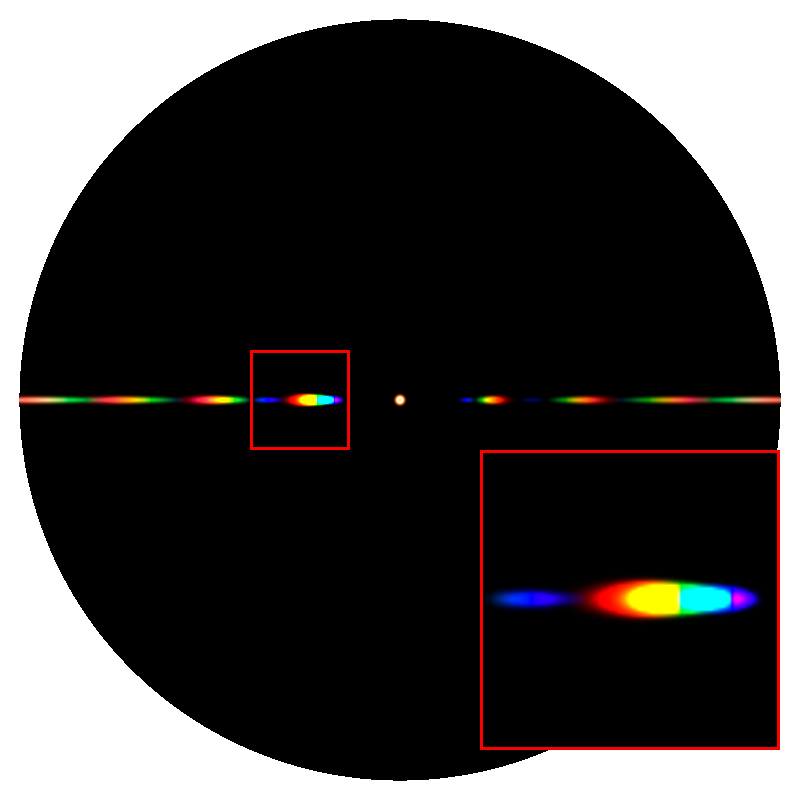
\includegraphics[scale=0.06]{results/taylorStepsVar/blaze/1.png}
    \label{fig:brdfmapsTaylorN1Blaze}
  }
~
  \subfigure[$N=2$]{
    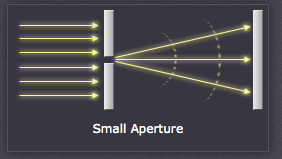
\includegraphics[scale=0.06]{results/taylorStepsVar/blaze/2.png}
    \label{fig:brdfmapsTaylorN2Blaze}
  }
~  
  \subfigure[$N=3$]{
    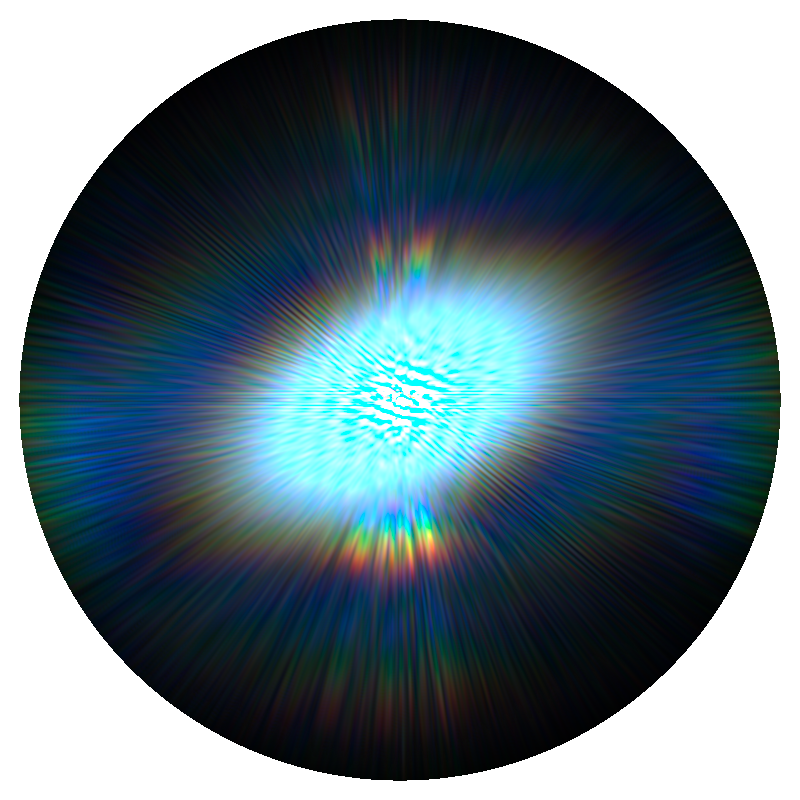
\includegraphics[scale=0.06]{results/taylorStepsVar/blaze/3.png}
    \label{fig:brdfmapsTaylorN3Blaze}
  }
~
  \subfigure[$N=4$]{
    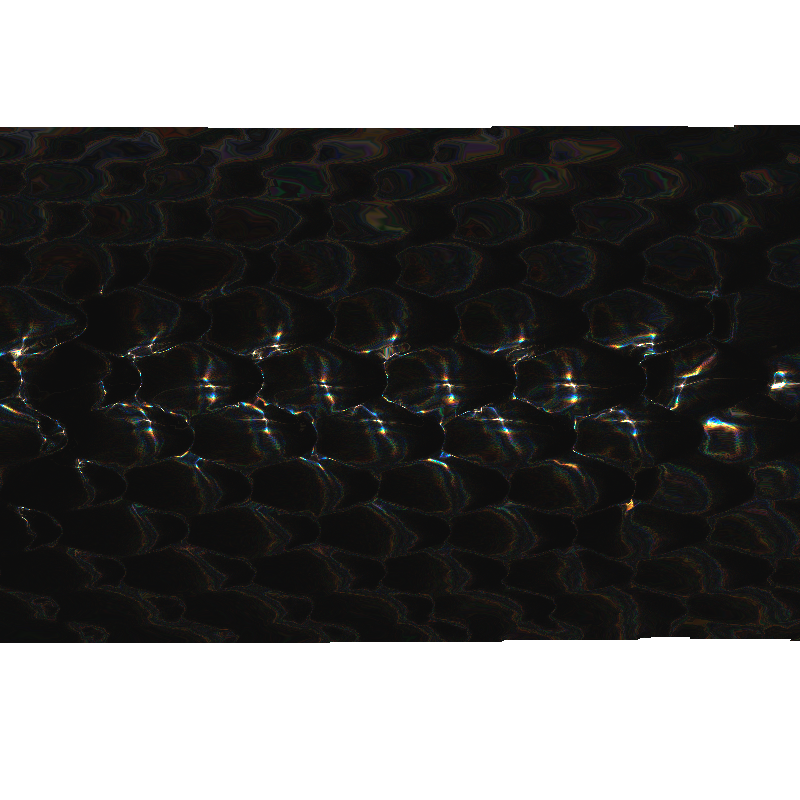
\includegraphics[scale=0.06]{results/taylorStepsVar/blaze/4.png}
    \label{fig:brdfmapsTaylorN4Blaze}
  }

  \subfigure[$N=5$]{
    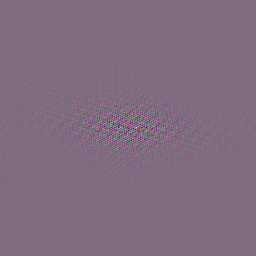
\includegraphics[scale=0.06]{results/taylorStepsVar/blaze/5.png}
    \label{fig:brdfmapsTaylorN5Blaze}
  }
~  
  \subfigure[$N=6$]{
    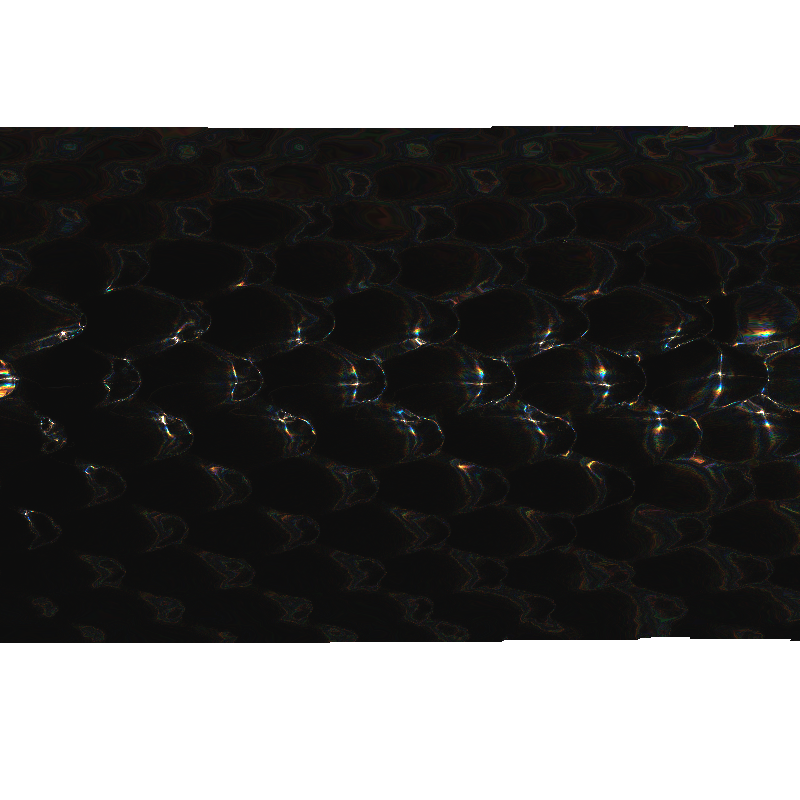
\includegraphics[scale=0.06]{results/taylorStepsVar/blaze/6.png}
    \label{fig:brdfmapsTaylorN6Blaze}
  }
~  
  \subfigure[$N=7$]{
    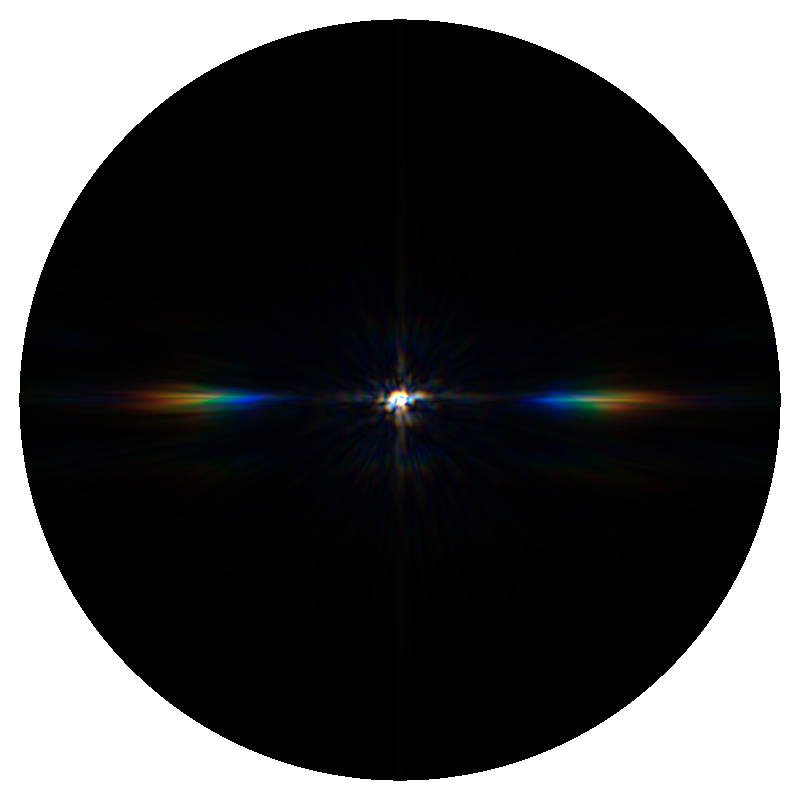
\includegraphics[scale=0.06]{results/taylorStepsVar/blaze/7.png}
    \label{fig:brdfmapsTaylorN7Blaze}
  }
~  
  \subfigure[$N=8$]{
    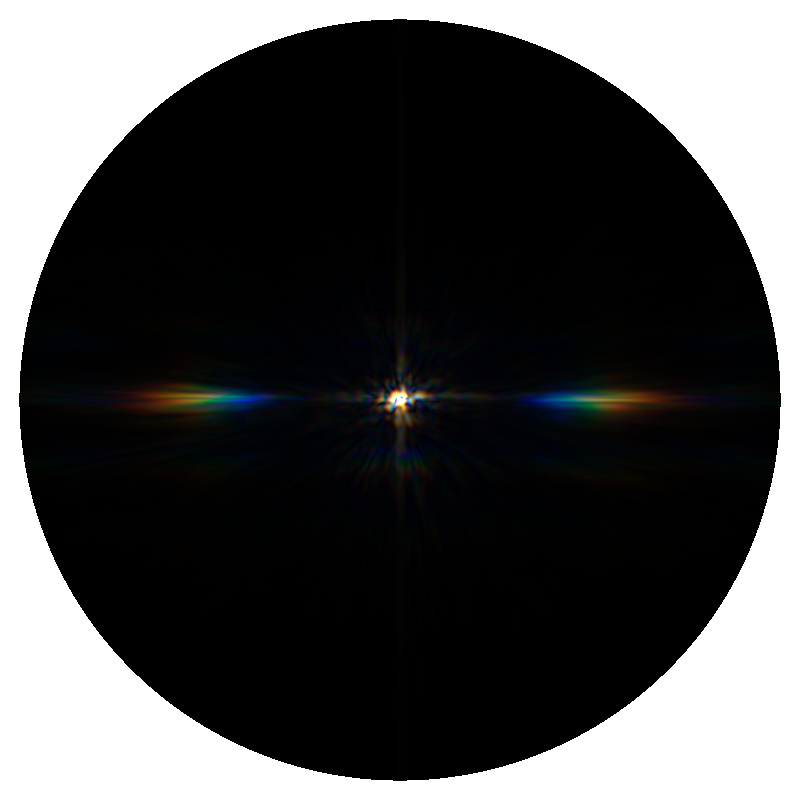
\includegraphics[scale=0.06]{results/taylorStepsVar/blaze/8.png}
    \label{fig:brdfmapsTaylorN8Blaze}
  }
~ 
  \subfigure[$N=9$]{
    \includegraphics[scale=0.06]{results/taylorStepsVar/blaze/9.png}
    \label{fig:brdfmapsTaylorN9Blaze}
  }
  
  
\caption{Blazed grating at $2.5 \mu m$: $N$ Taylor Iterations}
\label{fig:brdfmapstayloriterationsblaze}
\end{figure}

%taylor var elaphe
\begin{figure}[H]
  \centering
  \subfigure[$N=0$]{
    \includegraphics[scale=0.06]{results/taylorStepsVar/elaphe65/0.png}
    \label{fig:brdfmapsTaylorN0Elaphe65}
  }
~
  \subfigure[$N=1$]{
    \includegraphics[scale=0.06]{results/taylorStepsVar/elaphe65/1.png}
    \label{fig:brdfmapsTaylorN1Elaphe65}
  }
~
  \subfigure[$N=2$]{
    \includegraphics[scale=0.06]{results/taylorStepsVar/elaphe65/2.png}
    \label{fig:brdfmapsTaylorN2Elaphe65}
  }
~  
  \subfigure[$N=3$]{
    \includegraphics[scale=0.06]{results/taylorStepsVar/elaphe65/3.png}
    \label{fig:brdfmapsTaylorN3Elaphe65}
  }
~
  \subfigure[$N=4$]{
    \includegraphics[scale=0.06]{results/taylorStepsVar/elaphe65/4.png}
    \label{fig:brdfmapsTaylorN4Elaphe65}
  }

  \subfigure[$N=5$]{
    \includegraphics[scale=0.06]{results/taylorStepsVar/elaphe65/5.png}
    \label{fig:brdfmapsTaylorN5Elaphe65}
  }
~  
  \subfigure[$N=6$]{
    \includegraphics[scale=0.06]{results/taylorStepsVar/elaphe65/6.png}
    \label{fig:brdfmapsTaylorN6Elaphe65}
  }
~  
  \subfigure[$N=7$]{
    \includegraphics[scale=0.06]{results/taylorStepsVar/elaphe65/7.png}
    \label{fig:brdfmapsTaylorN7Elaphe65}
  }
~  
  \subfigure[$N=8$]{
    \includegraphics[scale=0.06]{results/taylorStepsVar/elaphe65/8.png}
    \label{fig:brdfmapsTaylorN8Elaphe65}
  }
~ 
  \subfigure[$N=9$]{
    \includegraphics[scale=0.06]{results/taylorStepsVar/elaphe65/9.png}
    \label{fig:brdfmapsTaylorN9Elaphe65}
  }
  
\caption{Elaphe grating at $65 \mu m$: $N$ Taylor Iterations}
\label{fig:brdfmapstayloriterationselaphe65}
\end{figure}


Figure $\ref{fig:brdfmapsxenodiffthetaiangles}$ shows the BRDF maps of the full lambda shading approach applied on the Xenopeltis snake shed, using different $\theta_i$ incident angles. When slightly moving the incident angle $\theta_i$, we can observe how the brdf map changes. For higher values of $\theta_i$ we start seeing diffraction color contribution on the right side of the BRDF map. 

% brdf maps xeno angles
\begin{figure}[H]
  \centering
  \subfigure[Xeno grating $\theta_i=0$]{
    \includegraphics[scale=0.12]{results/different_theta_i_angles/xenopeltis/xeno_t_i=0.png}
    \label{fig:brdfmapXenoti0}
  }
~
  \subfigure[Xeno grating $\theta_i=10$]{
    \includegraphics[scale=0.12]{results/different_theta_i_angles/xenopeltis/xeno_t_i=10.png}
    \label{fig:brdfmapXenoti10}
  }
~
  \subfigure[Xeno grating $\theta_i=20$]{
    \includegraphics[scale=0.12]{results/different_theta_i_angles/xenopeltis/xeno_t_i=20.png}
    \label{fig:brdfmapXenoti20}
  }
  
\caption{BRDF maps for Xeno grating: different $\theta_i$ angles}
\label{fig:brdfmapsxenodiffthetaiangles}
\end{figure}

\section{Snake surface geometries}
\label{sec:snakegeomrenderings}
In this section we are going to present our actual renderings simulating the effect of diffraction caused when a directional light source encounters different nano-scaled surfaces on a given curved snake mesh. We will see that diffraction colors change dramatically with changes in light direction, surface normals and viewing direction, which s typical for diffraction colors observed in nature. For rendering we are going to rely on our full wavelength space sampling approach. Unfortunately, this approach is rather slow and can barely be considered as being interactive performing. Nevertheless, we have introduced some optimizations in oder to become interactive in rendering, such as the $N_{min}, N_{max}$ approach, we are going to use this slow approach since this resembles the ground truth and therefore is the most accurate among all our presented approaches. As mentioned we are going to render diffraction on a given snake mesh. Note that we actually just have one particular mesh, for all our renderings we are going to use the same snake mesh which has been produced by 3d scanning an Elpahe snake species, consisting of 11696 vertices and 22950 faces. The reason for that is that it was hard to get a Xenopeltis snake ready for being 3d scanned. In addition, the micro-geometry is highly similar among snake species, it is the geometry of the nano-structures that are highly different among species and that cause the snake to be or not be iridescent. So, even Xenopeltis would not give you very different geometry than Elaphe. Table $\ref{tab:hardwarespecifications}$ lists the system specifications of the machine I used in order to produce the rendered images.

\begin{table}[H]
  \centering
  \begin{tabular}{|r|l|}
    \hline
    Processor & Intel i7 CPU 970 @ 3.20 GHz (12 CPUs) \\
    Memory & 12288 MB RAM \\
    Graphics Card & GeForce GTX 770 \\
    \hline  
  \end{tabular}
\caption[Hardware Specifications]{Hardware specifications of the machine which produced rendered results. Statistics are provided using the tool NVIDIA Geforce Experience.}
\label{tab:hardwarespecifications}
\end{table}

Figure $\ref{fig:renderingdifferentsnankegratings}$ shows renderings produced by the full lambda sampling approach applied on a snake shaped mesh for different given input patches. Due do the fact that a Blazed grating has its maximum intensity for a certain direction and the geometry of the snake mesh is curved which means non-flat, we can expect rather less diffraction color contribution like shown in figure $\ref{fig:renderingelaphegrating}$. Differently for our other two gratings, Elaphe and Xenopeltis. For both renderings, we can see color contribution despite the effect of diffraction whereas we see much less colorful patterns for Elpahe $\ref{fig:renderingelaphegrating}$ than for Xenopeltis $\ref{fig:renderingxenograting}$. This also corresponds to the reality, considering the figure $\ref{fig:snakespecies}$ as a reference. The nano-scaled surface structure of the species Elapse as shwon in figure $\ref{fig:elpahegratingpatch}$ does not look that regular under the electron scanning microscope. This is why it is much less iridescent than the other specie. Xeno has a brownish body with no pattern that makes the iridescence more spectacular than on Ellaphe. 
 
\begin{figure}[H]
  \centering
  \subfigure[Blazed grating]{
    \includegraphics[scale=0.12]{results/snakerenderings/compars/blaze.png}
    \label{fig:renderingblazegrating}
  }
~
  \subfigure[Elaphe grating]{
    \includegraphics[scale=0.12]{results/snakerenderings/compars/elaphe65.png}
    \label{fig:renderingelaphegrating}
  }
~
  \subfigure[Xeno grating]{
    \includegraphics[scale=0.12]{results/snakerenderings/compars/xeno65.png}
    \label{fig:renderingxenograting}
  }
  
\caption{Diffraction of different snake skin gratings rendered on a snake geometry}
\label{fig:renderingdifferentsnankegratings}
\end{figure}

Figure $\ref{fig:renderingelaphe65}$ contains a summary-collection of subfigures for rendering the effect of diffraction produced by the full lambda shading approach with all its required components, applied on our snake mesh, using the Elaphe nano-scaled surface structure. Subfigure $\ref{fig:renderingelaphe65dt}$ shows the final diffraction color-contribution result with texture-blending. We only see little diffraction color contribution in this subfigure which resembles quite well to the reality as shown in figure $\ref{fig:elpahespecies}$. In subfigure $\ref{fig:renderingelaphe65ns}$ we see the light cone in order to show the direction of the light source besides the rendered results. Subfigure $\ref{fig:renderingelaphe65ft}$ is a sample Fourier image of Elpahe's nanosclae surface structure $\ref{fig:renderingelaphe65ns}$.

\begin{figure}[H]
  \centering
  \subfigure[Diffraction Patten]{
    \includegraphics[scale=0.2]{results/snakerenderings/elaphe65/1.png}
    \label{fig:renderingelaphe65dp}
  }
~
  \subfigure[Diffraction + Texture]{
    \includegraphics[scale=0.2]{results/snakerenderings/elaphe65/2.png}
    \label{fig:renderingelaphe65dt}
  }

  \subfigure[Texture + Lightdir]{
    \includegraphics[scale=0.12]{results/snakerenderings/elaphe65/3.png}
    \label{fig:renderingelaphe65tl}
  }
~
  \subfigure[Nanostructure]{
    \includegraphics[scale=0.10]{results/snakerenderings/elaphe65/4.png}
    \label{fig:renderingelaphe65ns}
  }
~ 
  \subfigure[Fourier Transform]{
    \includegraphics[scale=0.52]{results/snakerenderings/elaphe65/5.png}
    \label{fig:renderingelaphe65ft}
  }
  
\caption{Diffraction for Elaphe snake skin}
\label{fig:renderingelaphe65}
\end{figure}


Like in the previous figure this figure $\ref{fig:renderingxeno65}$ also shows a summary-collection of subfigures for the effect of diffraction with all its involved components but this time for the Xenopeltis snake surface. For texture blending we use the same texture like we used for Elaphe. For Xenopeltis see quite a lot color contribution due the phenomenon of diffraction like shown in figure $\ref{fig:renderingXeno65DT}$. Comparing this to a real image $\ref{fig:xenospeicies}$ we notice much resemblance regarding the reflectance strength and colorful pattern.

\begin{figure}[H]
  \centering
  \subfigure[Diffraction Patten]{
    \includegraphics[scale=0.2]{results/snakerenderings/xeno65/1.png}
    \label{fig:renderingXeno65DP}
  }
~
  \subfigure[Diffraction + Texture]{
    \includegraphics[scale=0.2]{results/snakerenderings/xeno65/2.png}
    \label{fig:renderingXeno65DT}
  }

  \subfigure[Texture + Lightdir]{
    \includegraphics[scale=0.12]{results/snakerenderings/xeno65/3.png}
    \label{fig:renderingXeno65TL}
  }
~
  \subfigure[Nanostructure]{
    \includegraphics[scale=0.075]{results/snakerenderings/xeno65/4.png}
    \label{fig:renderingXeno65NS}
  }
~ 
  \subfigure[Fourier Transform]{
    \includegraphics[scale=0.52]{results/snakerenderings/xeno65/5.png}
    \label{fig:renderingXeno65FT}
  }
  
  
  
\caption{Diffraction for Xeno snake skin}
\label{fig:renderingxeno65}
\end{figure}

Figure $\ref{fig:renderingdifferentzoomlevelselaphe}$ shows the diffraction pattern of a Elaphe snake shed for different zoom levels for fixed incident light and viewing direction using the full lambda sampling approach. From those different close up perspectives it would appear the complexity of the colorful diffraction pattern.

\begin{figure}[H]
  \centering
  \subfigure[$zoom = 0.1$]{
    \includegraphics[scale=0.2]{results/snakerenderings/zoomIn/elaphe65/0.1.png}
    \label{fig:renderingZoomElaphe01}
  }
~
  \subfigure[$zoom = 0.2$]{
    \includegraphics[scale=0.2]{results/snakerenderings/zoomIn/elaphe65/0.2.png}
    \label{fig:renderingZoomElaphe02}
  }
  
  \subfigure[$zoom = 0.5$]{
    \includegraphics[scale=0.2]{results/snakerenderings/zoomIn/elaphe65/0.5.png}
    \label{fig:renderingZoomElaphe05}
  }
~
  \subfigure[$zoom = 1.0$]{
    \includegraphics[scale=0.2]{results/snakerenderings/zoomIn/elaphe65/1.png}
    \label{fig:renderingZoomElaphe1}
  }
  
  \subfigure[$zoom = 1.5$]{
    \includegraphics[scale=0.2]{results/snakerenderings/zoomIn/elaphe65/1.5.png}
    \label{fig:renderingZoomElaphe15}
  }
~
  \subfigure[$zoom = 2.0$]{
    \includegraphics[scale=0.2]{results/snakerenderings/zoomIn/elaphe65/2.png}
    \label{fig:renderingZoomElaphe2}
  }
  
\caption{Diffraction on Elaphe snake skin grating: Different camera zoom levels}
\label{fig:renderingdifferentzoomlevelselaphe}
\end{figure}


Figure $\ref{fig:renderingelaphelightrotations6}$ shows how the diffraction pattern changes when slightly moving the incident light direction. Which gives us an impression what kind of complex, perspective-dependent pattern the phenomenon of diffraction may cause.

% first 3 move along x, next 3 move along y
\begin{figure}[H]
  \centering
  \subfigure[$(-3.3130, 0.0, -0.9999)$]{
    \includegraphics[scale=0.12]{results/snakerenderings/rotateLight/elaphe65/moveX/2.png}
    \label{fig:renderingElapheRotX2}
  }
~
  \subfigure[$(-0.1989, 0.0, -0.9799)$]{
    \includegraphics[scale=0.12]{results/snakerenderings/rotateLight/elaphe65/moveX/4.png}
    \label{fig:renderingElapheRotX4}
  }
~
  \subfigure[$(-0.3897, 0.0, -0.9208)$]{
    \includegraphics[scale=0.12]{results/snakerenderings/rotateLight/elaphe65/moveX/6.png}
    \label{fig:renderingElapheRotX6}
  }
  
  \subfigure[$(0.0995, 0.0993, -0.9900)$]{
    \includegraphics[scale=0.12]{results/snakerenderings/rotateLight/elaphe65/moveY/2.png}
    \label{fig:renderingElapheRotY2}
  }
~
  \subfigure[$(0.0995, 0.2940, -0.9505)$]{
    \includegraphics[scale=0.12]{results/snakerenderings/rotateLight/elaphe65/moveY/4.png}
    \label{fig:renderingElapheRotY4}
  }
~
  \subfigure[$(0.0995, 0.4770, -0.8731)$]{
    \includegraphics[scale=0.12]{results/snakerenderings/rotateLight/elaphe65/moveY/6.png}
    \label{fig:renderingElapheRotY6}
  }
  
  
\caption{Diffraction on Elaphe snake skin grating: Different light directions}
\label{fig:renderingelaphelightrotations6}
\end{figure}

Figure $\ref{fig:experimentelaphe65}$ shows a photo of an experimental setup for demonstrating the effect of diffraction using a Elpahe snake grating. The exact parameters for the experimental setup are unknown. Nevertheless this image gives us an impression of how close our model is to the reality comparing it with our simulated results since we notice similar diffraction patterns for our simulated results using an Elaphe snake shed. 

\begin{figure}[H]
  \includegraphics[scale=0.2]{results/experiment/elaphe/g2.png}
  \caption{Diffraction Elaphe: experimental setup}
  \label{fig:experimentelaphe65}
\end{figure}

